
\section{Determinación de las distribuciones de sustentación básica y adicional} \label{sec:distribucion_lift}

El coeficiente de sustentación de una ala a lo largo de la envergadura es
\begin{equation} \label{eq:cl_general}
    C_l (y) = C_{l,\alpha} \left(\alpha - \alpha_i (y) - \alpha_{l0}(y) + \varepsilon(y) \right)
\end{equation}
con $\alpha_i(y)$ el ángulo de ataque inducido por el \emph{downwash} \cite{mccormick_1}. Es conveniente dividir el $C_l(y)$ en dos contribuciones. La primera es la sustentación básica $\left( C_{l_b}(y) \right)$. Depende de la forma en planta del ala, del ángulo de ataque de sustentación nula $\left( \alpha_{l0}(y) \right)$, de la torsión $\left( \varepsilon(y) \right)$ y su integral a lo largo de la envergadura es nula, \ie, 
\begin{equation} \label{eq:cl_basico}
     C_{l_b} \Rightarrow 
     I_b = \frac{1}{S} \int_{-b/2}^{b/2} C_{l_b}(y) \, c(y) \, d y = 0
\end{equation}
La segunda es la sustentación adicional. Solamente depende de la forma en planta del ala sin torsión y su integral es unitaria, 
\begin{equation} \label{eq:cl_adicional}
     C_{l_a} \Rightarrow 
    I_a = \frac{1}{S} \int_{-b/2}^{b/2} C_{l_a}(y) \, c(y) \, d y = 1 
\end{equation}
La distribución de sustentación en cualquier condición de vuelo se puede escribir como
\begin{equation} \label{eq:cl_seccion_distribuciones}
    C_l(y) = C_{l_b}(y) + C_{l_a}(y) \, C_L
\end{equation}
Las distribuciones $C_{l_b}(y)$ y $C_{l_a}(y)$ son propiedades del ala. Conociendo $C_l(y)$ y $C_L$ en dos condiciones de vuelo distintas $1$ y $2$, se puede plantear un sistema de ecuaciones compatible determinado de dimensión 2. Resolviendo para ambas distribuciones, se consigue
\begin{gather}
    C_{l_b}(y) = \frac{C_{l2}(y) \, C_{L1} - C_{l1}(y) \, C_{L2}}{C_{L1} - C_{L2}} \label{eq:calculo_clb} \\
    C_{l_a}(y) = \frac{C_{l1}(y) - C_{l2}(y)}{C_{L1} - C_{L2}} \label{eq:calculo_cla} 
\end{gather}

Numéricamente se calcula la distribución de sustentación local y el coeficiente de sustentación del ala con una discretización de $N = 200$ paneles. Usando \eqref{eq:calculo_clb} y \eqref{eq:calculo_cla}, se obtienen las distribuciones básica y adicional. En la figura \ref{fig:lift_distribution} se representan ambas distribuciones a lo largo de la envergadura.

\begin{figure}[ht]
    \centering
    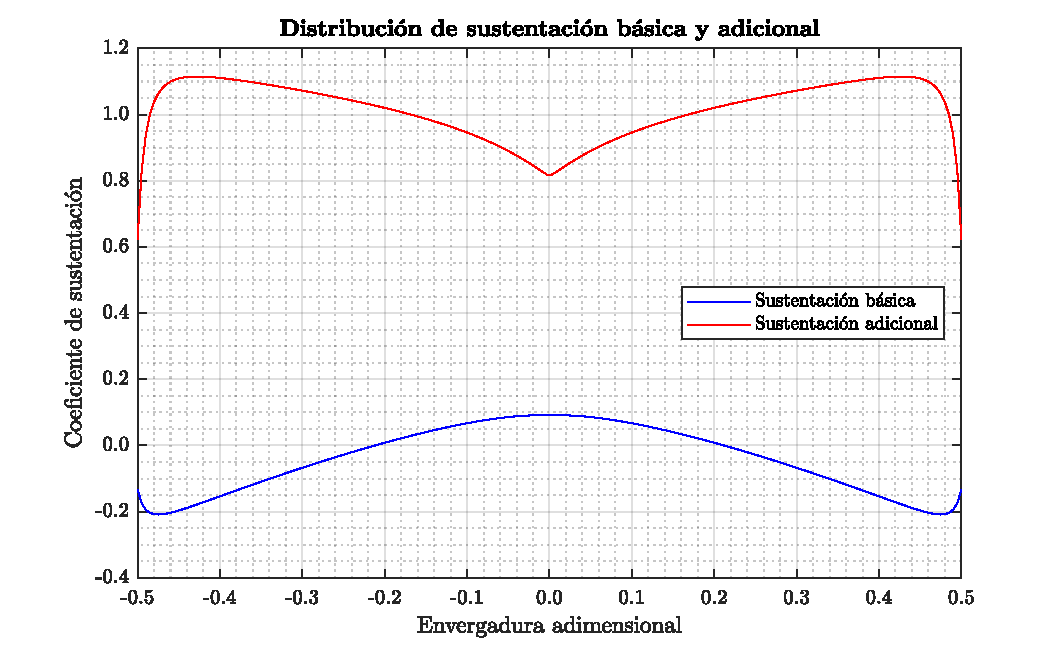
\includegraphics[width=\linewidth]{imagenes/distribucion_lift/lift_distribution.pdf}
    \caption{Distribuciones de coeficiente de sustentación básica $\left( C_{l_b} \right)$ y adicional $\left( C_{l_a} \right)$ a lo largo de la envergadura del ala.}
    \label{fig:lift_distribution}
    \vspace{-4mm}
\end{figure}

Para ambas distribuciones se calcula la integral numérica según \eqref{eq:cl_basico} y \eqref{eq:cl_adicional}, usando la regla del trapecio. Para la distribución $C_{l_b}$ se obtiene $I_b = -0.0236$. Para la distribución $C_{l_a}$ se obtiene $I_a = 0.9879$. En ambos casos el error es inferior al $2.5\%$, por consiguiente se trata de una buena aproximación.  

Como se ha comentado, la torsión geométrica solo influye en la distribución de sustentación básica. En la figura \ref{fig:torsion_basic_lift} se representa la distribución de sustentación básica para diversas torsiones geométricas en punta de ala, calculadas con $N = 200$ paneles.

\begin{figure}[h]
    \centering
    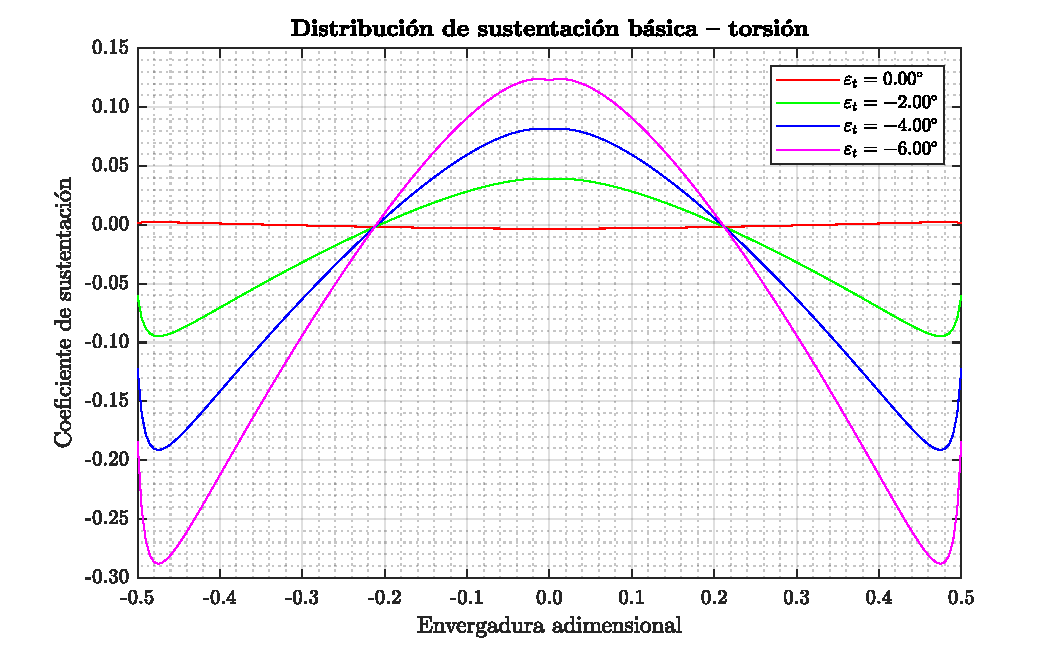
\includegraphics[width=\linewidth]{imagenes/distribucion_lift/torsion_basic_lift.pdf}
    \caption{Distribuciones de coeficiente de sustentación básica $\left( C_{l_b} \right)$ a lo largo de la envergadura del ala, para torsiones geométricas $\left( \varepsilon_t \right)$ entre $-6\degrees$ y $0 \degrees$.}
    \label{fig:torsion_basic_lift}
    \vspace{-4mm}
\end{figure}

\noindent
Cuando la torsión geométrica en punta de ala disminuye, los extremos relativos de la distribución $C_{l_b}(y)$ crecen. Para $\varepsilon_t = 0$, $C_{l_b}(y)$ es aproximadamente constante. Por el contrario, con $\varepsilon_t = -6\degrees$ la variación es significativa. Cuando $\varepsilon_t$ disminuye, el ángulo de ataque que ven las secciones también disminuye, pudiendo llegar a darse $C_l(y)$ negativo. Esto mismo se refleja en las distribuciones de $C_{l_b}(y)$. Al modificar la distribución de sustentación, la sustentación total así como el centro de presiones varían. De este modo, para un determinado $C_L$ de diseño, se puede trabajar la distribución de sustentación y conseguir que el momento alrededor del CG sea nulo.





